\subsection{Aufbau}
    Die meisten Silizium-basierten Solarzellen haben den gleichen
    grundsätzlichen Aufbau und nur geringe Unterschiede wie das Muster
    der vorderen Kontakte.
    \begin{figure}[H]
        \centering
        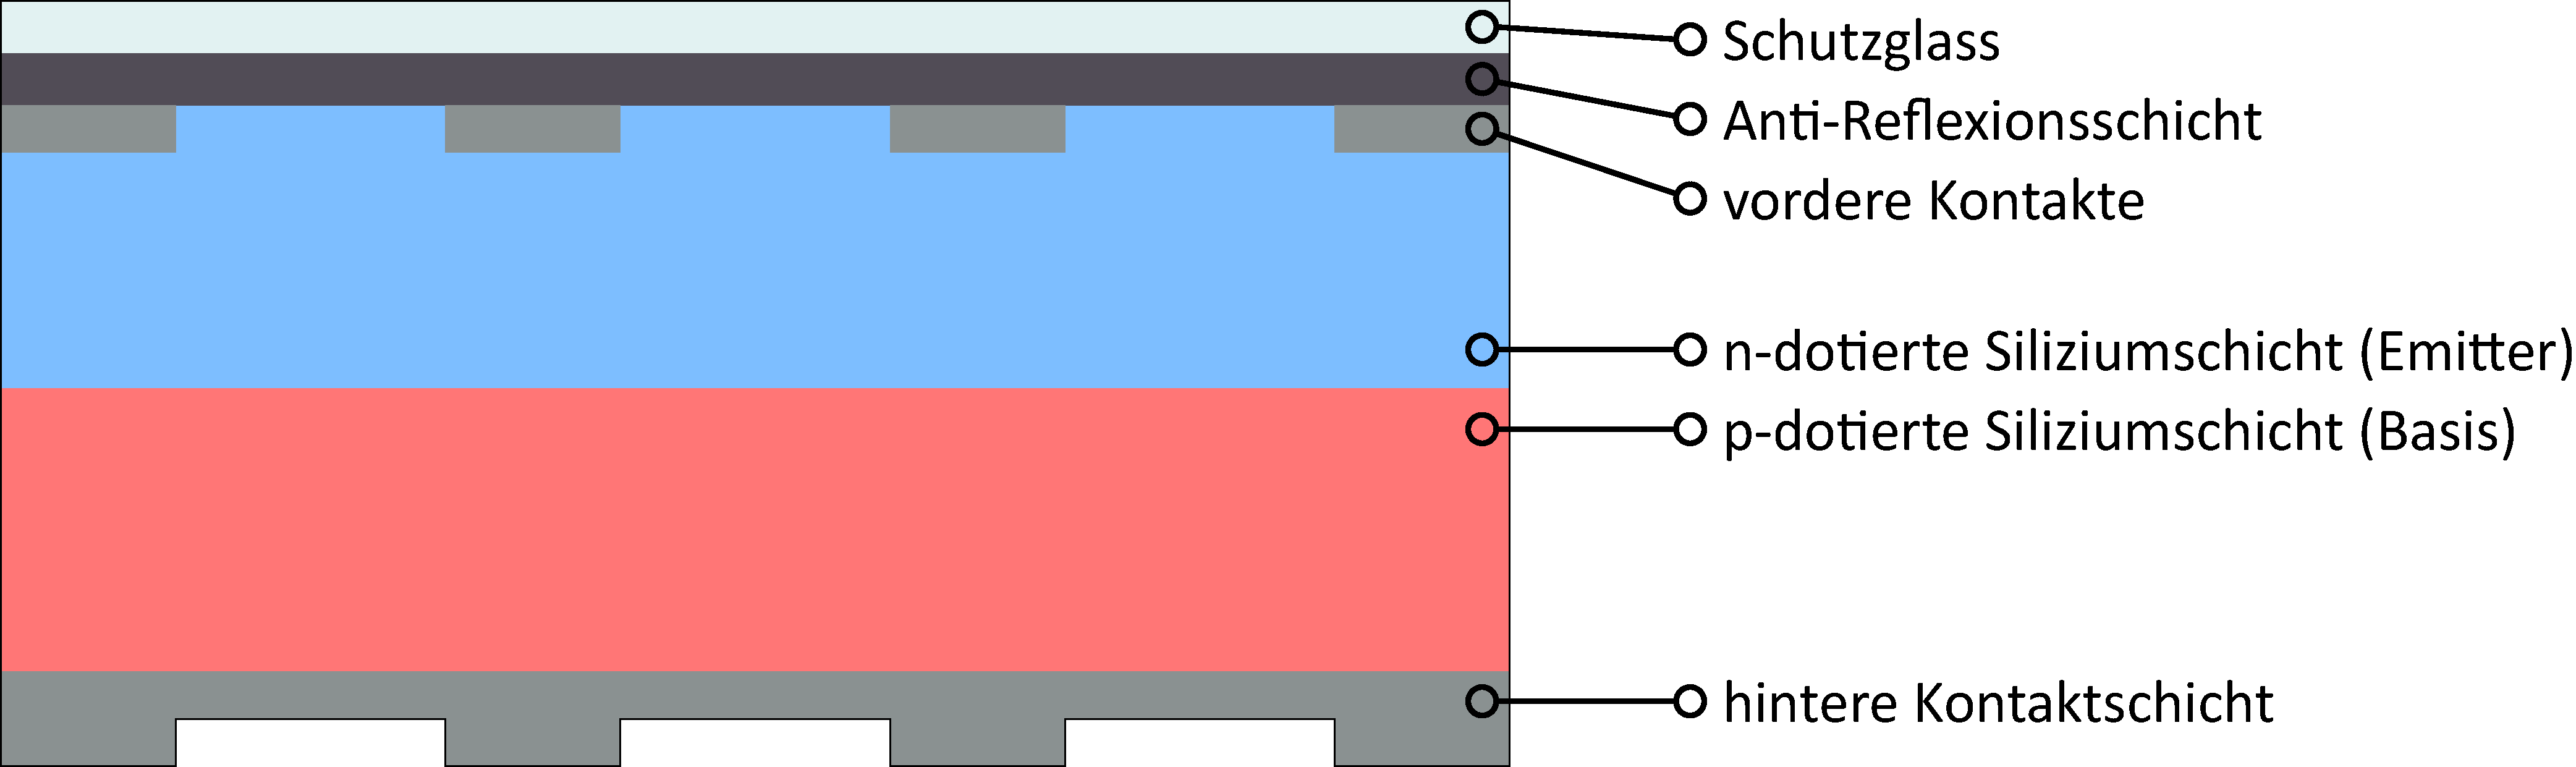
\includegraphics[width=1.0\linewidth]{solarzelle_schnitt.pdf}
        \caption{Grunlegender Aufbau einer Silizium-basierten Solarzelle}
    \end{figure}
    Die Dotierung der Schichten beschreibt einen
    Prozess mit bei dem der Siliziumkristall mit Unreinheiten besetzt
    wird um die Halbleiter-Eigenschaften hervorzurufen. Silizium hat
    4 Valenzelektronen und bildet somit Kristallstrukturen durch Kovalente
    Bindungen. Durch das dotieren mit Elektronen mit mehr als 4
    Valenzelektronen entsteht eine n-dotierte Schicht, bei dotieren mit
    Atomen mit weniger als 4 Valenzelektronen eine p-dotierte Schicht.

\subsection{Funktionsweise}
    Wenn eine Solarzelle von Photonen mit einer Wellenlängen von maximal 1110nm
    getroffen wird welche nicht reflektiert werden, können diese bei
    Interaktion mit Atomen in den p- und n-dotierten Schichten Elektronen-
    Loch-Paare erzeugen.
    \begin{figure}[H]
        \centering
        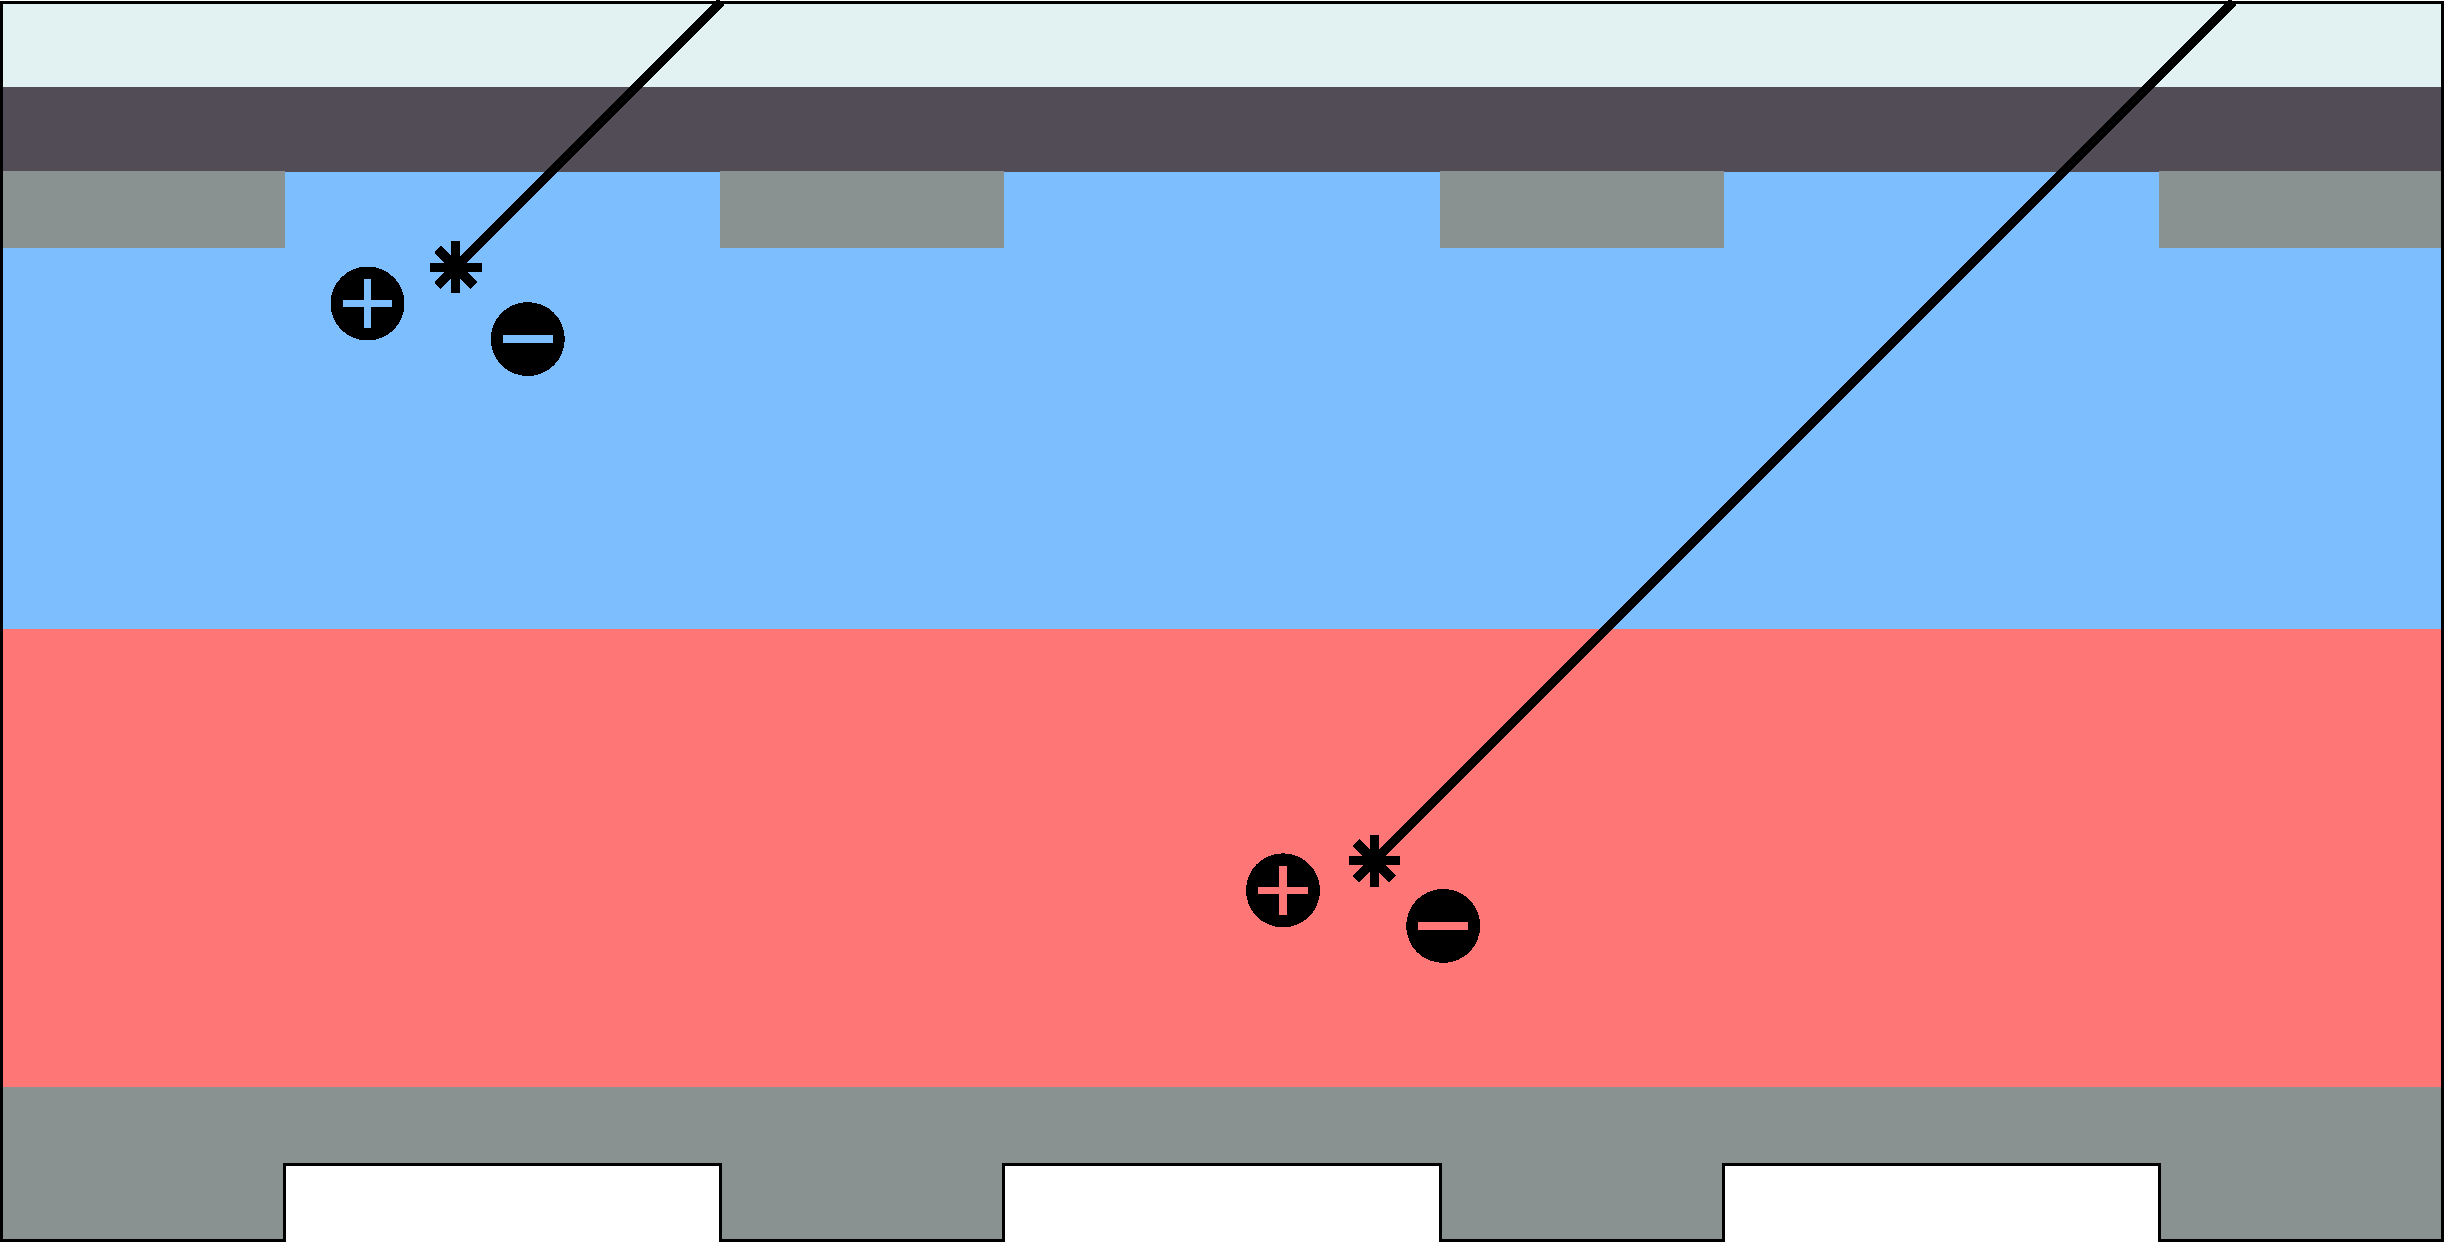
\includegraphics[width=0.65\linewidth]{solarzelle_schnitt_schritt1.pdf}
        \caption{Bildung Elektronen-Loch-Paare}
    \end{figure}
    Durch die Halbleiter-Eigentschaften der Solarzelle bewegen sich befreiten
    Elektronen in Richtung der der n-dotierten Schicht (blau) und Löcher in
    Richtung der p-dotierten Schicht (rot).
    \begin{figure}[H]
        \centering
        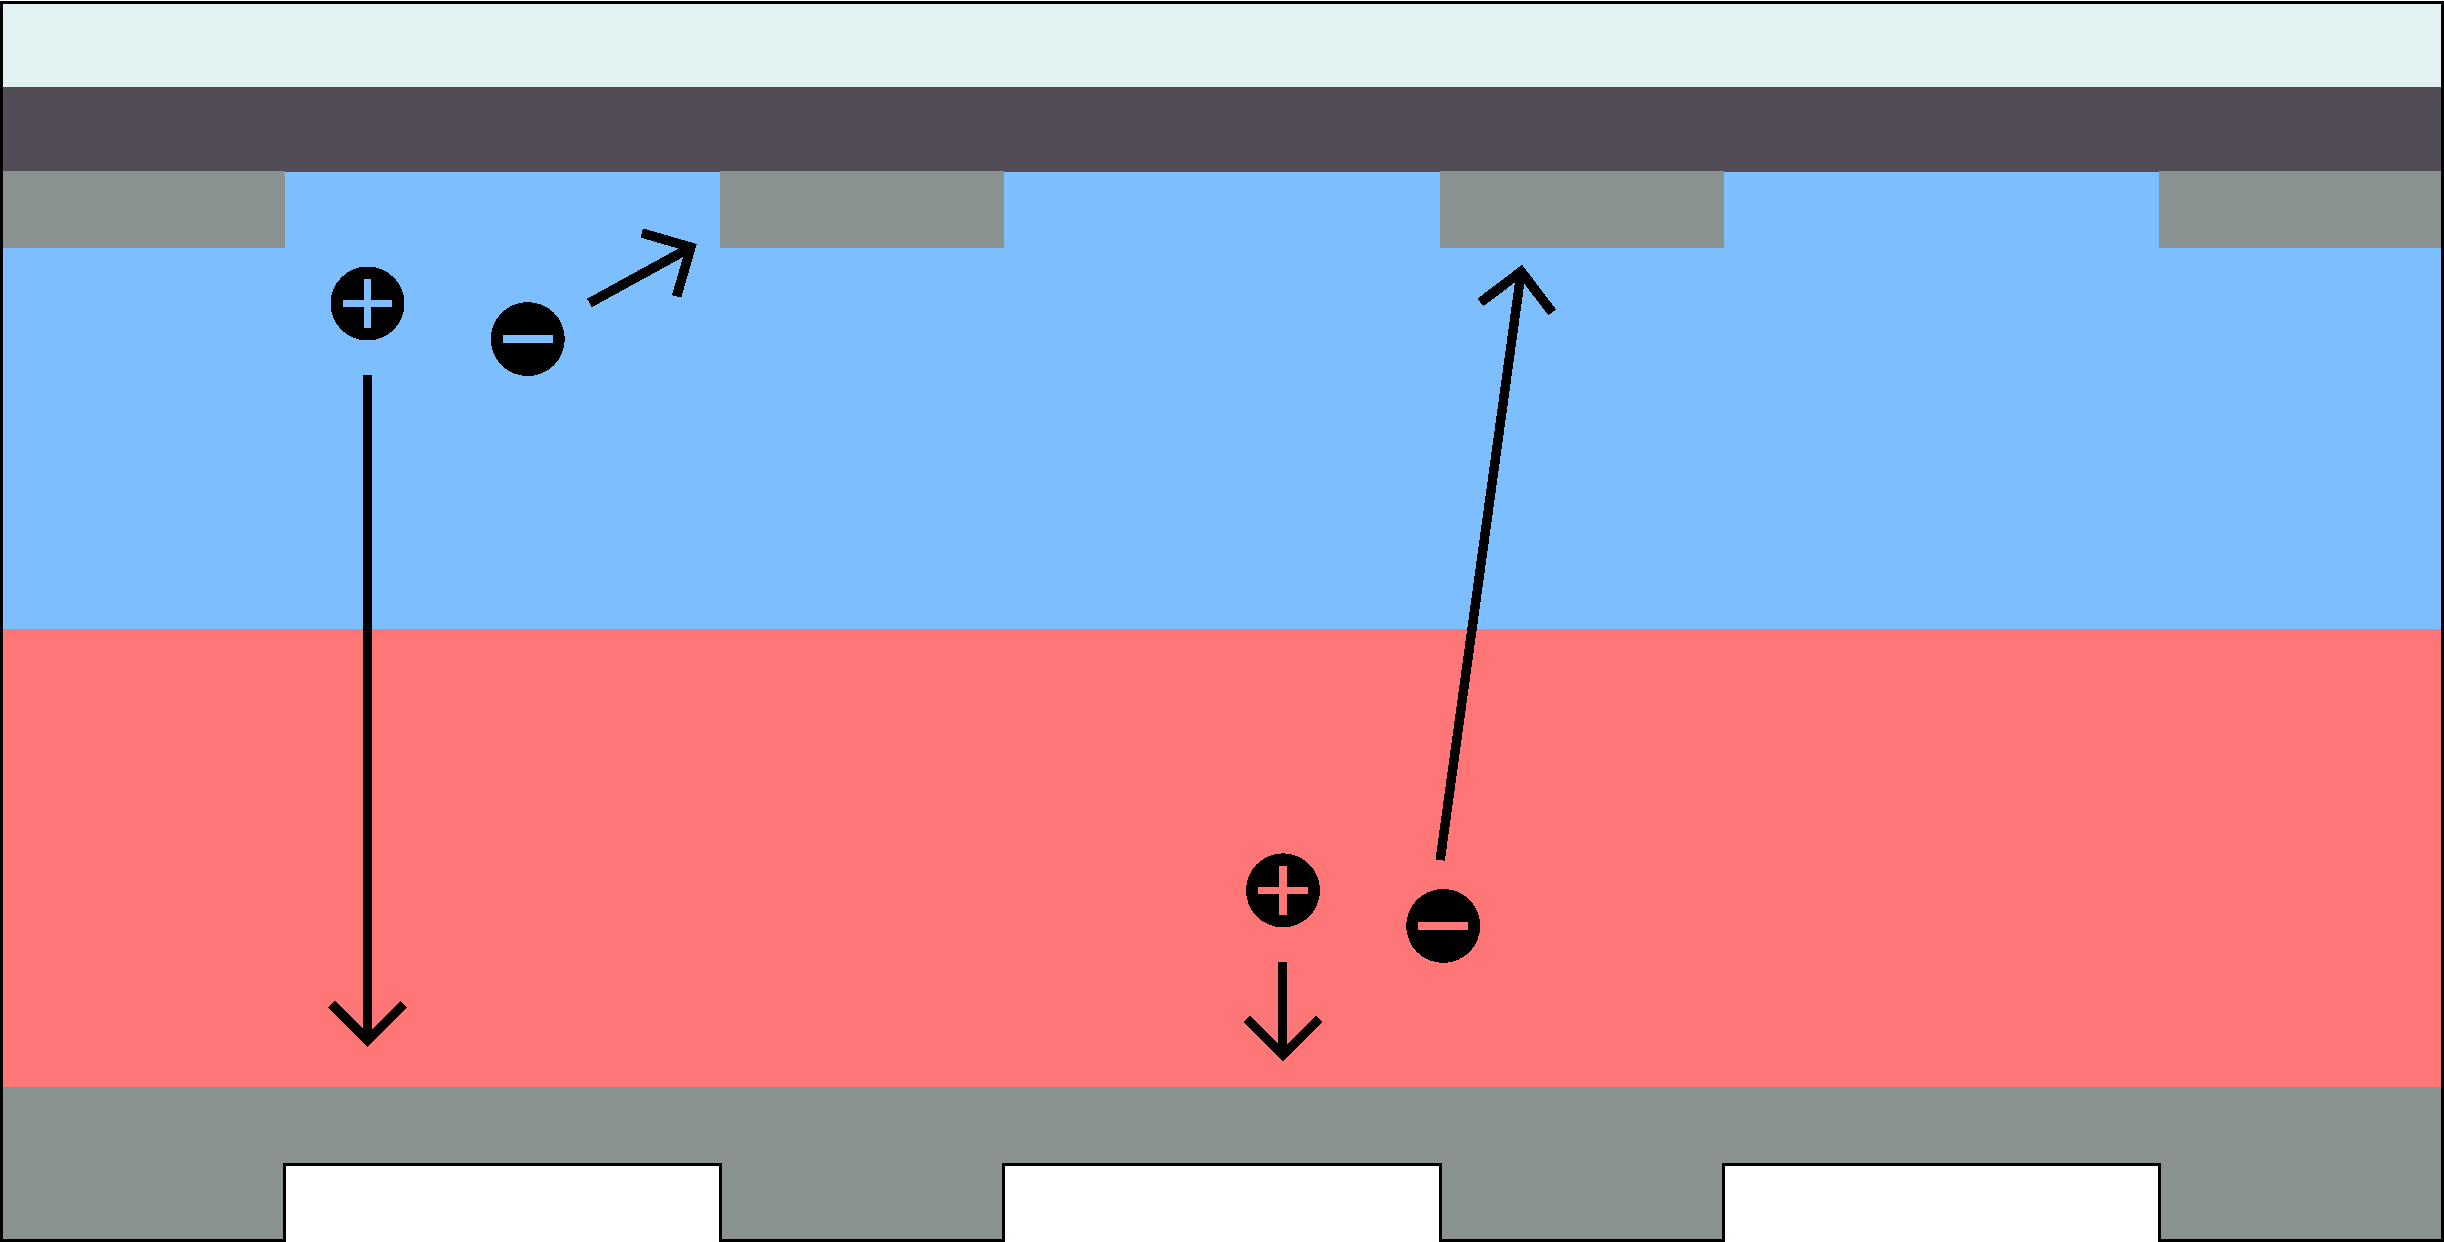
\includegraphics[width=0.65\linewidth]{solarzelle_schnitt_schritt2.pdf}
        \caption{Bildung des Photostroms}
    \end{figure}
    Der dabei entstehende Strom nennt sich Photostrom und die dabei Entstehende
    Potentialdifferenz erzeugt eine Spannung welche bei Anlegen eines externen
    Verbrauchers an die oberen und unteren Kontakte einen Messbaren Strom
    erzeugt.
    \begin{figure}[H]
        \centering
        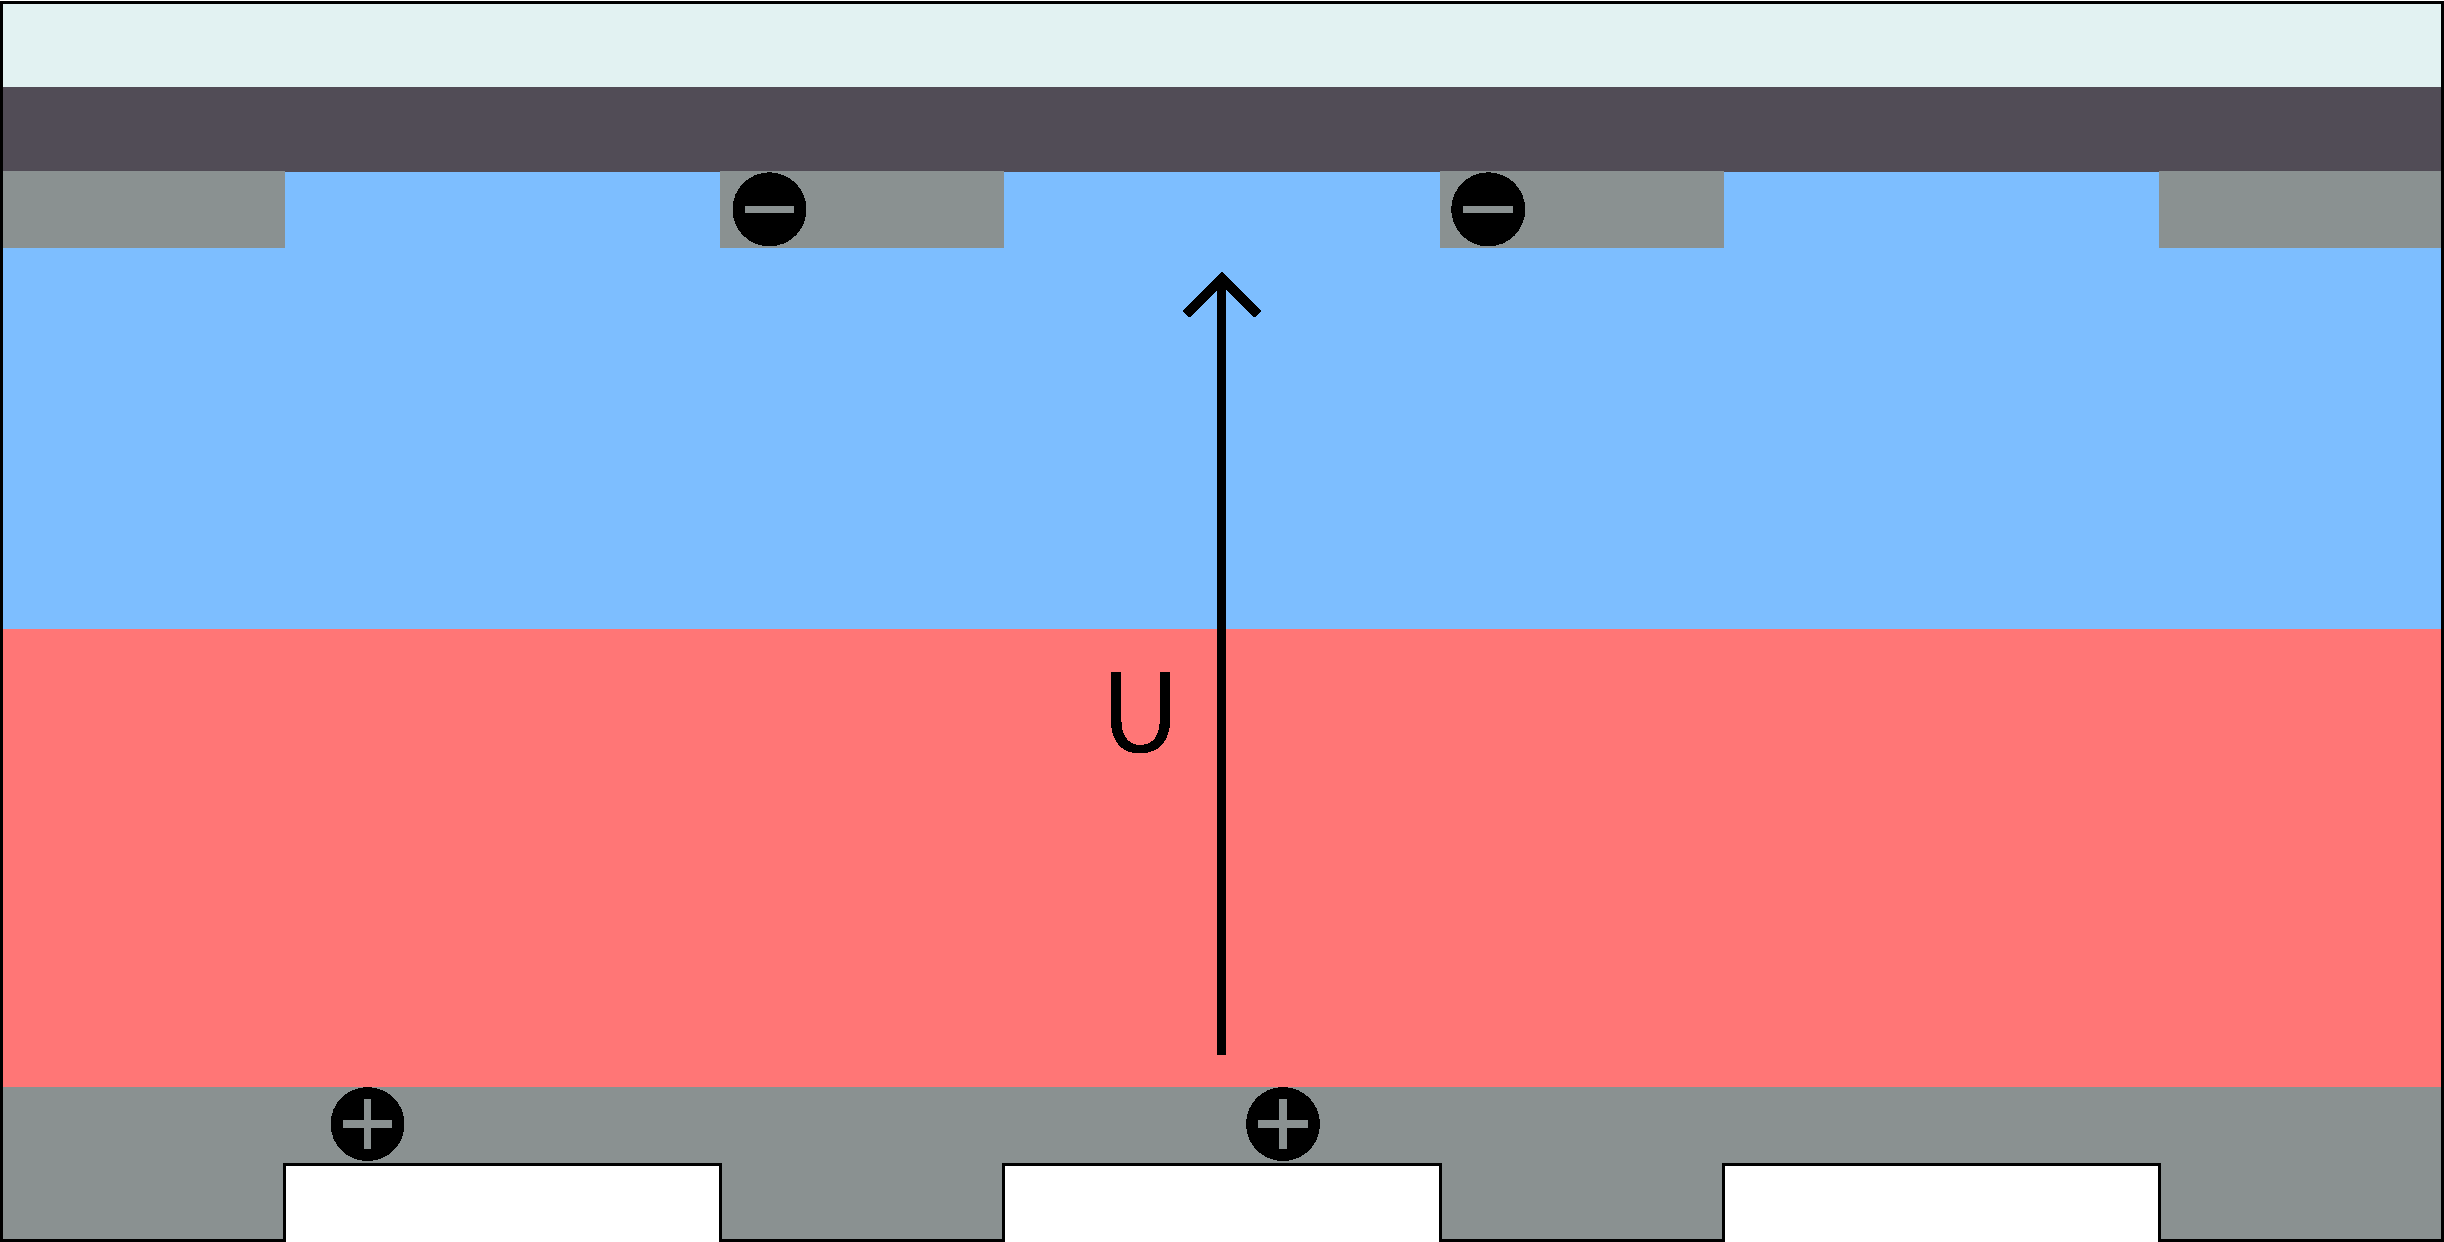
\includegraphics[width=0.65\linewidth]{solarzelle_schnitt_schritt3.pdf}
        \caption{Entstehen einer messbaren Spannung}
    \end{figure}
    Erst wenn ein externer Verbraucher angeschlossen ist, bewegen sich
    Elektronen und Löcher zu den nahe gelegenen Kontakten und dann über den
    Verbraucher zurück in die jeweiligen Sichten.

\subsection{Vorteile}
    Nach der Installation von Solarzellen ist kein Rohmaterial oder
    Energiezufluss benötigt um Energie zu produzieren. Dadurch das
    Solarzellen keine beweglichen oder kontaktintensiven Teile besitzen
    brauchen sie beinahe keine Wartung und sind sehr robust
    \cite{SolarMaintenance}.

\subsection{Nachteile}
    Solarzellen sind Anfällig für Temperaturschwankungen, bei höheren
    Temperaturen sinkt die Effizienz von Solarzellen. Die durschnittliche
    Energieeffizienz von Solarzellen liegt bei etwa 15\% bis 20\% (unter
    Laborkonditionen) \cite{SolarEfficiency}, das heißt das rund 85\% bis 80\%
    der aufgefangenen Sonnenenergie entweder reflektiert oder in Wärme
    umgewandelt wird welche wiederum die Effizienz verringert (die überflüssige
    thermische Energie kann allerdings zur Effizienzsteigferung beitragen
    \cite{PhotovoltaicPrinciples} Chapter 3, Page 22/24).
    % TODO: carbon footprint etc